This section describe Ascent's primary abstractions and surveys its general capabilities.
%
Ascent organizes its capabilities into five types of in situ tasks, which
it refers to as \textbf{actions}.
%
Its five actions are:
\begin{itemize}
\item \textbf{Pipelines} transform data from one form to another.
%
\item \textbf{Scenes} render images.
%
\item \textbf{Extracts} are used to move data out of Ascent, i.e., to file I/O or to another framework.
%
\item \textbf{Queries} provide quantitative summarizations of the data.
%
\item \textbf{Triggers} adapt when other actions are executed, based on the conditions of the simulation.
%
\end{itemize}

These actions are highly interoperable, and Ascent can employ multiple actions of the same type
at once.
%
Consider the following example of Ascent doing in situ analysis on an input data set, $D$,
for a given cycle of a simulation.
%
Ascent begins by applying an isosurfacing operation to $D$ to make a new data set $D'$ (pipeline).
%
It then applies a trigger to $D'$ --- it takes the surface area of the isosurface (query) and compares
the total area with the area from the previous time it was executed.
%
If the total area has changed by more than 5\%, then Ascent would render an image of $D'$ (scene)
and also save the original data set $D$ to disk (extract).
%
Going beyond this example, it is possible to have multiple triggers, arbitrary conditions for
the triggers (queries or otherwise), as well as many pipelines, scenes, and extracts.
%
Figure~\ref{fig:ascent_example} shows an example of this, specifically two pipelines and two extracts.

\begin{figure}
\centering
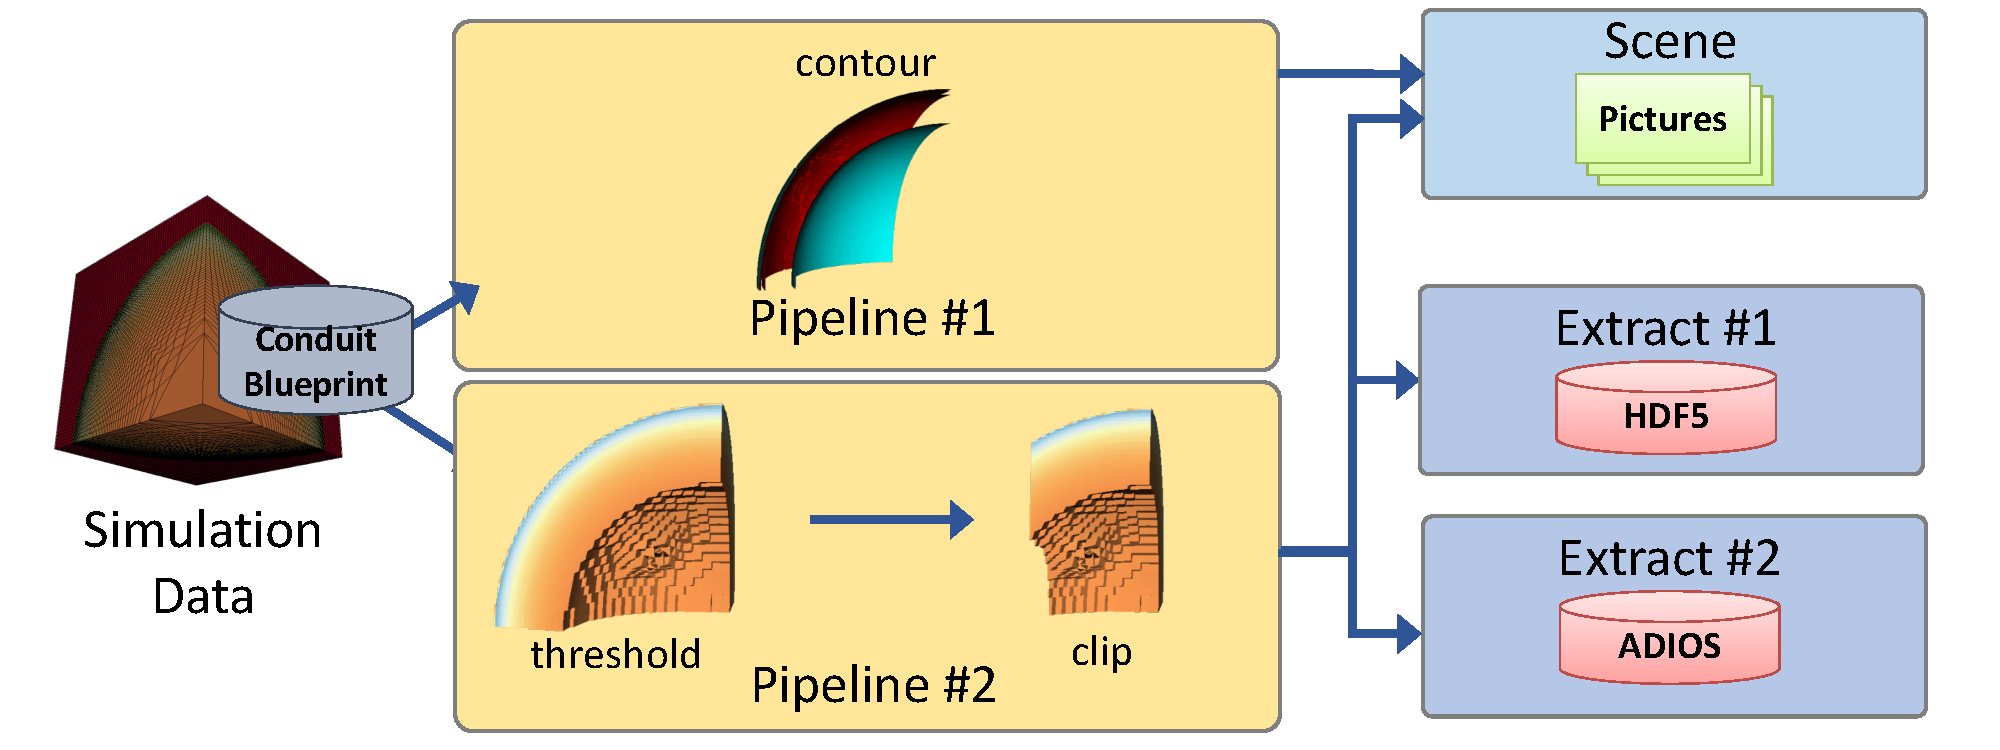
\includegraphics[width=\textwidth]{images/ascent_actions_diagram.pdf}
\caption{\label{fig:ascent_example} An example of how Ascent actions can be combined.
In this example, simulation data is acquired from Conduit/Blueprint (see \S\ref{sec:API}),
and that data is relayed into two pipelines (labeled \#1 and \#2). 
The first pipeline applies a contour operation, while the second
applies threshold and clip operations.
%
The results of these pipelines are used in multiple ways.
A scene uses both pipelines as input, while two extracts use only the second pipeline
as input, outputting using two different I/O libraries.}
\end{figure}

%Currently supported filters include:

%\fix{I feel like this section should take the following form:
%1) what the concept is and 2) what are our current capabilities}

\subsection{Pipelines}

Pipelines allows users to describe a series of data transformations, also known as filters,
to execute on simulation data.
%
%These data transformations are sometimes referred to as filters in other
%frameworks (like VTK~\cite{VTK}), and 
Figure~\ref{fig:ascent_example} shows
typical filters for visualization: contour, threshold, and clip.
%Figure~\ref{img:pipelines} shows two examples of pipelines.
%%
%Pipeline \#1 creates contours from a simulation field, and pipeline \#2
%thresholds cells that are within a scalar range then applies a clipping operation.
%
Ascent allows users can define an arbitrary number of pipelines.
%
In terms of inputs and outputs, the input to a pipeline is either
the simulation data or another pipeline, and the outputs of a pipeline
can go to scenes, extracts, and queries.  
%
Further, triggers can make use of pipelines, and their relationship is discussed further
in \S\ref{sec:ascent:triggers}.

%
%The default source of pipelines, and all other actions, is the data
%published by the simulation, but all actions can consume the results
%of declared pipelines, including other pipelines.

%\begin{figure}
%\centering
%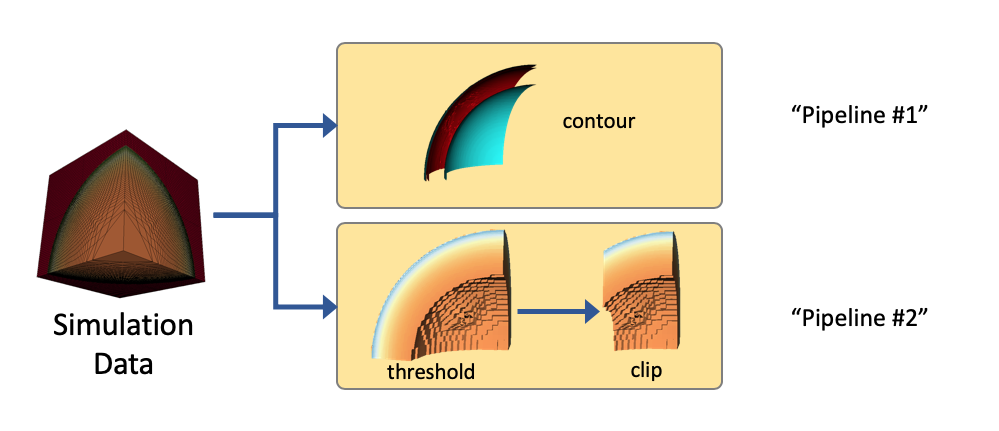
\includegraphics[width=0.6\textwidth]{images/pipelines}
%\caption{\label{img:pipelines} Examples pipelines that transforms simulation data via visualization operators.}
%\end{figure}

Notable filters currently supported by Ascent include:
\begin{multicols}{2}
\begin{itemize}
\item Clipping
\item Contour
\item Histogram
\item Isovolume
\item Particle Advection
\item Statistics
\item Slice
\item Threshold
\end{itemize}
\end{multicols}

There are also filters that create new fields: Divergence, Gradient, Logarithm, Q-Criterion, Vector Magnitude, and Vorticity.
%
Finally, Ascent contains two specific-to-in-situ filters that 
reduce data size significantly enough that it can be saved to disk and explored post hoc: 
Lagrangian Flow and Sampling.


\subsection{Scenes}

Scenes allow users to specify how images are rendered.
%
Each scene consists of one or more plots, and Ascent supports volume,
pseudocolor, and mesh plots.
%
Plot types contain parameters such scalar fields, color tables, and scalar ranges,
in addition to the name of the pipeline to consume.
%
Scenes also can contain zero or more \textit{renders}, which contain
camera specifications, image dimensions, background and
foreground colors, annotation controls.
%
Ascent creates a default camera based on bounding box of the data set and
is always facing the data set.
%
Renders inherit the default camera parameters, which simplifies creating
cameras that actually look at the data set.
%
Ascent also provides simple controls to rotate the camera on the
sphere circumscribing the data set, although the user is free to set all
camera parameters explicitly.
%
Additionally, scenes can create Cinema~\cite{AhrensCinema} databases that
create a large set of images that can be explored after the simulation.

Currently supported plots include:
\begin{itemize}
\item Psuedocolor
\item Mesh
\item Volume
\item Radiograph
\end{itemize}

\subsection{Extracts}
Extracts are an escape hatch in Ascent that enables data to be sent
outside of Ascent.
%
Extracts can be as simple a saving data to HDF5 files or can be a gateway
to a larger workflow.
Extracts provide a means to link codes integrated with Ascent to other tools.
%
While, Ascent visualization covers many visualization use cases,
Ascent does not have the long tail of functionality that tools like ParaView or VisIt provide, which
were built over many years of development.
%
Through extracts, Ascent can pass data directly to ParaView Catalyst~\cite{Catalyst}.
%
Another example of using extracts to provide additional functionality is the
ADIOS~\cite{Lofstead2008} extract, which allows ascent to link to in-transit workflows.

Ascent supports connections to the Python ecosystem through the Python and
Jupyter extracts~\cite{CyrusISAV,Jupyter}.
%
Python extracts execute custom analysis code provided by the user, and the
Jupyter extracts allow for incoming Jupyter notebooks connections from a web
browser.

Jupyter notebooks is a promising direction for in situ.
%
One of in situ's greatest weaknesses is the it's reliance on a priori
knowledge, and one strategy to mitagate this weakness is interactivity.
%
Through the Jupyter notebook interface, users can pause a running simulation
and interact with the data.
%
Additionally, Jupyter widgets enable fast prototyping of domain specific
GUIs.

Currently supported extracts include:
\begin{itemize}
\item ADIOS (beta)
\item Babel Flow~\cite{babelflow}
\item Jupyter Notebooks
\item ParaView Catalyst
\item Python
\end{itemize}

\subsection{Queries}
\label{action_queries}
Queries in Ascent allow users to ask questions about simulation data,
or data from pipelines, through a Python like language.
%
Queries provide access to data summarization functions and access to the
current state of the simulation..
%
Examples include min-max queries, statistics, cell locations,
and probability distributions.
%
Queries are executed each time Ascent is called, and the resulting time
history can be saved, accessed by the simulation, or accessed in other
expressions.

Queries can be as simple as calling a function that returns the current simulation cycle
and storing it into a variable.
%
More complex queries can calculate the amount of entropy of a field.
%
The expression language that backs queries can perform math operations,
call functions, and evaluate conditionals.
%
Since queries are stored into named identifiers, subsequent queries
can build on the results of other queries, allowing for complex combinations.

Examples of queries include:
\begin{itemize}
\item $cycle()$
\item $max(field('pressure'))$
\item $entropy(histogram(field('gyre'), num\_bins=128))$
\end{itemize}
%Listing~\ref{simple_query} shows the declaration of a query that returns
%the current simulation cycle and stores it into a variable identifier \textit{cycle},
%and Listing~\ref{complex_query} shows a more complex example of a query that
%calculates the entropy of a simulation field.
%\begin{lstlisting}[language=Python,caption={Examples of querying the simulation cycle}, label={simple_query}]
%# add a simple query expression (q1)
%queries["q1/params/expression"] = "cycle()"
%queries["q1/params/name"] = "cycle"
%\end{lstlisting}
%

%
%
%\begin{lstlisting}[language=Python,caption={A more complex example of queries in Ascent}, label={complex_query}]
%# add a more complex query expression (q2)
%queries["q2/params/expression"] = "entropy(histogram(field('gyre'), num_bins=128))"
%queries["q2/params/name"] = "entropy_of_gyre"
%\end{lstlisting}

\subsection{Triggers}
\label{sec:ascent:triggers}
Traditional in situ actions execute every $X$ simulation cycles, this presents
two related problems.
%
First, if the analysis is expensive, then the total cost of the action may exceed
what a user is willing to pay, e.g., adding a 50\% overhead on top of the simulation.
%
Second, if the analysis called infrequently, then the feature or event that the analysis is
trying to capture could easily be missed.
%
Triggers address these issues by coupling inspection routines with analysis, and a
potentially costly analysis only executes when user defined precondition is met.
%
Ideally, inspection routines are cheap and can be called every cycle, while the analysis
that are ``triggered'' can cost more.

Ascent triggers builds on the queries and expression support introduced in
Section~\ref{action_queries}, and the trigger condition can be any conditional
expression.
%
When the condition evaluates to true, the trigger fires, executing a user provided
set of actions, which can be any Ascent action.
%
Triggers can be used to execute actions for debugging purposes(i.e., saving data to
a file when invalid values are found) or rendering images when a large
change is found(i.e., when the max value of a field exceeds a threshold from the
previous value).
%
When an event can be expressed in these terms, triggers are a powerful tool for
maximizing constrained resources in situ.

Example of triggers include:
\begin{itemize}
\item $cycle() > 100 and cycle() < 200$
\item $max(field('pressure')) > 100.0$
\item $magnitude(max(field('braid')).position - vector(0,0,0)) > 0$
\end{itemize}
